\documentclass[letterpaper]{article} % DO NOT CHANGE THIS
\usepackage{aaai24}  % DO NOT CHANGE THIS
\usepackage{times}  % DO NOT CHANGE THIS
\usepackage{helvet}  % DO NOT CHANGE THIS
\usepackage{courier}  % DO NOT CHANGE THIS
\usepackage[hyphens]{url}  % DO NOT CHANGE THIS
\usepackage{booktabs}
\usepackage{graphicx} % DO NOT CHANGE THIS
\urlstyle{rm} % DO NOT CHANGE THIS
\def\UrlFont{\rm}  % DO NOT CHANGE THIS
\usepackage{natbib}  % DO NOT CHANGE THIS AND DO NOT ADD ANY OPTIONS TO IT
\usepackage{caption} % DO NOT CHANGE THIS AND DO NOT ADD ANY OPTIONS TO IT
\frenchspacing  % DO NOT CHANGE THIS
\setlength{\pdfpagewidth}{8.5in} % DO NOT CHANGE THIS
\setlength{\pdfpageheight}{11in} % DO NOT CHANGE THIS
\usepackage{algorithm}
\usepackage{algorithmic}

\usepackage{newfloat}
\usepackage{listings}
\DeclareCaptionStyle{ruled}{labelfont=normalfont,labelsep=colon,strut=off} % DO NOT CHANGE THIS
\lstset{%
	basicstyle={\footnotesize\ttfamily},% footnotesize acceptable for monospace
	numbers=left,numberstyle=\footnotesize,xleftmargin=2em,% show line numbers, remove this entire line if you don't want the numbers.
	aboveskip=0pt,belowskip=0pt,%
	showstringspaces=false,tabsize=2,breaklines=true}
\floatstyle{ruled}
\newfloat{listing}{tb}{lst}{}
\floatname{listing}{Listing}


\setcounter{secnumdepth}{0} %May be changed to 1 or 2 if section numbers are desired.



\title{Relation Extraction from News Articles (RENA): A Tool for Epidemic Surveillance}
\author{
    Jaeff Hong\equalcontrib\textsuperscript{\rm 2}, Duong Dung\equalcontrib\textsuperscript{\rm 1}, Danielle Hutchinson\textsuperscript{\rm 1}, Zubair Akhtar\textsuperscript{\rm 1}, Rosalie Chen\textsuperscript{\rm 1}, Rebecca Dawson\textsuperscript{\rm 1}, Aditya Joshi\footnote{Corresponding author}\textsuperscript{\rm 2}, Samsung Lim\textsuperscript{\rm 1 \rm 3}, C Raina MacIntyre\textsuperscript{\rm 1} and Deepti Gurdasani\textsuperscript{\rm 1 \rm 4 \rm 5}, \\
}
\affiliations{
    \textsuperscript{\rm 1}Kirby Institute, University of New South Wales, Sydney, Australia\\
 \textsuperscript{\rm 2}School of Computer Science \& Engineering, University of New South Wales, Sydney, Australia\\
\textsuperscript{\rm 3}School of Civil and Environmental Engineering, University of New South Wales, Sydney, Australia\\
 \textsuperscript{\rm 4}William Harvey Research Institute, Queen Mary University of London, London, UK\\
 \textsuperscript{\rm 5}School of Medicine, University of Western Australia, WA, Australia\\

 jaeff.hong@gmail.com, \{duong.dung, danielle.hutchinson, zubair.akhtar, rosalie.chen, rebecca.dawson, aditya.joshi, s.lim, r.macintyre, d.gurdasani\}@unsw.edu.au

}

\iffalse
\title{My Publication Title --- Single Author}
\author {
    Author Name
}
\affiliations{
    Affiliation\\
    Affiliation Line 2\\
    name@example.com
}
\fi

\iffalse
\title{My Publication Title --- Multiple Authors}
\author {
    First Author Name\textsuperscript{\rm 1},
    Second Author Name\textsuperscript{\rm 2},
    Third Author Name\textsuperscript{\rm 1}
}
\affiliations {
    \textsuperscript{\rm 1}Affiliation 1\\
    \textsuperscript{\rm 2}Affiliation 2\\
    firstAuthor@affiliation1.com, secondAuthor@affilation2.com, thirdAuthor@affiliation1.com
}
\fi


\usepackage{bibentry}

\begin{document}

\maketitle

\begin{abstract}
Relation Extraction from News Articles (RENA) is a browser-based tool designed to extract key entities and their semantic relationships in English language news articles related to infectious diseases. Constructed using the React framework, this system presents users with an elegant and user-friendly interface. It enables users to input a news article and select from a choice of two models to generate a comprehensive list of relations within the provided text. As a result, RENA allows real-time parsing of news articles to extract key information for epidemic surveillance, contributing to EPIWATCH, an open-source intelligence-based epidemic warning system.
\end{abstract}

\section{Introduction}
Online news websites are a valuable source of information about real-world events with several potential applications. One such application is the use of news articles for text-based epidemic intelligence~\cite{joshi2019survey}. EPIWATCH is an open-source intelligence-based early warning system for epidemics that parses vast amounts of data in real-time to build a structured repository of data to study changing trends in diseases and syndromes, geographically, over time~\cite{macintyre2023artificial}. A relevance classifier selects news articles from multiple sources~\cite{?}, which are then reviewed by expert analysts daily to generate structured data such as name of disease, number of cases and so on. This structured information allows identification of potential outbreaks earlier than traditional surveillance systems, alerting health authorities, thereby allowing for quicker outbreak response, and preventing further spread, ultimately saving lives~\cite{puca2020using}.

The manual task of extracting structured information from news articles maps to the natural language processing (NLP) task of relation extraction~\cite{banko2008tradeoffs, kumar2017survey}. Our browser-based tool, \textit{Relation Extraction from News Articles (RENA)}, uses decoder-only foundation models (also known as `large language models', \textit{i.e.}, LLMs) to extract semantic relations in infectious disease-related news articles in the English language\footnote{With appropriate choice of foundation models, RENA can be extended to languages other than English. We are interested in doing so.} at the document level. When an epidemiologist enters a news article, RENA extracts a list of entities and relations present in the article. This streamlines an automated process for epidemiologists and researchers who need a method to acquire a large congregate of structured relations from their selected article. By making use of RENA, they can be aided in their research without having to read a large set of news articles or delve into manual data curation.

Whilst many previous relation extraction (RE) tasks have focused on the sentence level, it is evident that many relations exist between different sentences, presenting another challenge in extracting relations at the document level~\cite{xu2021document}. We assume a simplistic definition of a relation: a relation connects exactly two entities. In the context of epidemic intelligence, the sentence `A patient died due to COVID-19 today' results in the relations \{death number: '1', relation: 'death of', infectious disease: COVID-19'\}, \{death number: '1', relation: 'occurred on', event date: 'today'\} and \{infectious disease: COVID-19, relation: 'occurred on', event date; 'today'\}. In this specific case, if two relations are identified, the third can be inferred.

RENA can be used by epidemiologists, public health officials and teachers or students of public health to extract information from news articles of interest. While the utility of RENA is for infectious disease-related epidemic intelligence, it can potentially be used for news articles across domains and application areas, including journalists/news publishers who want to verify and investigate information across multiple sources.
\begin{figure*}[h]
\centering
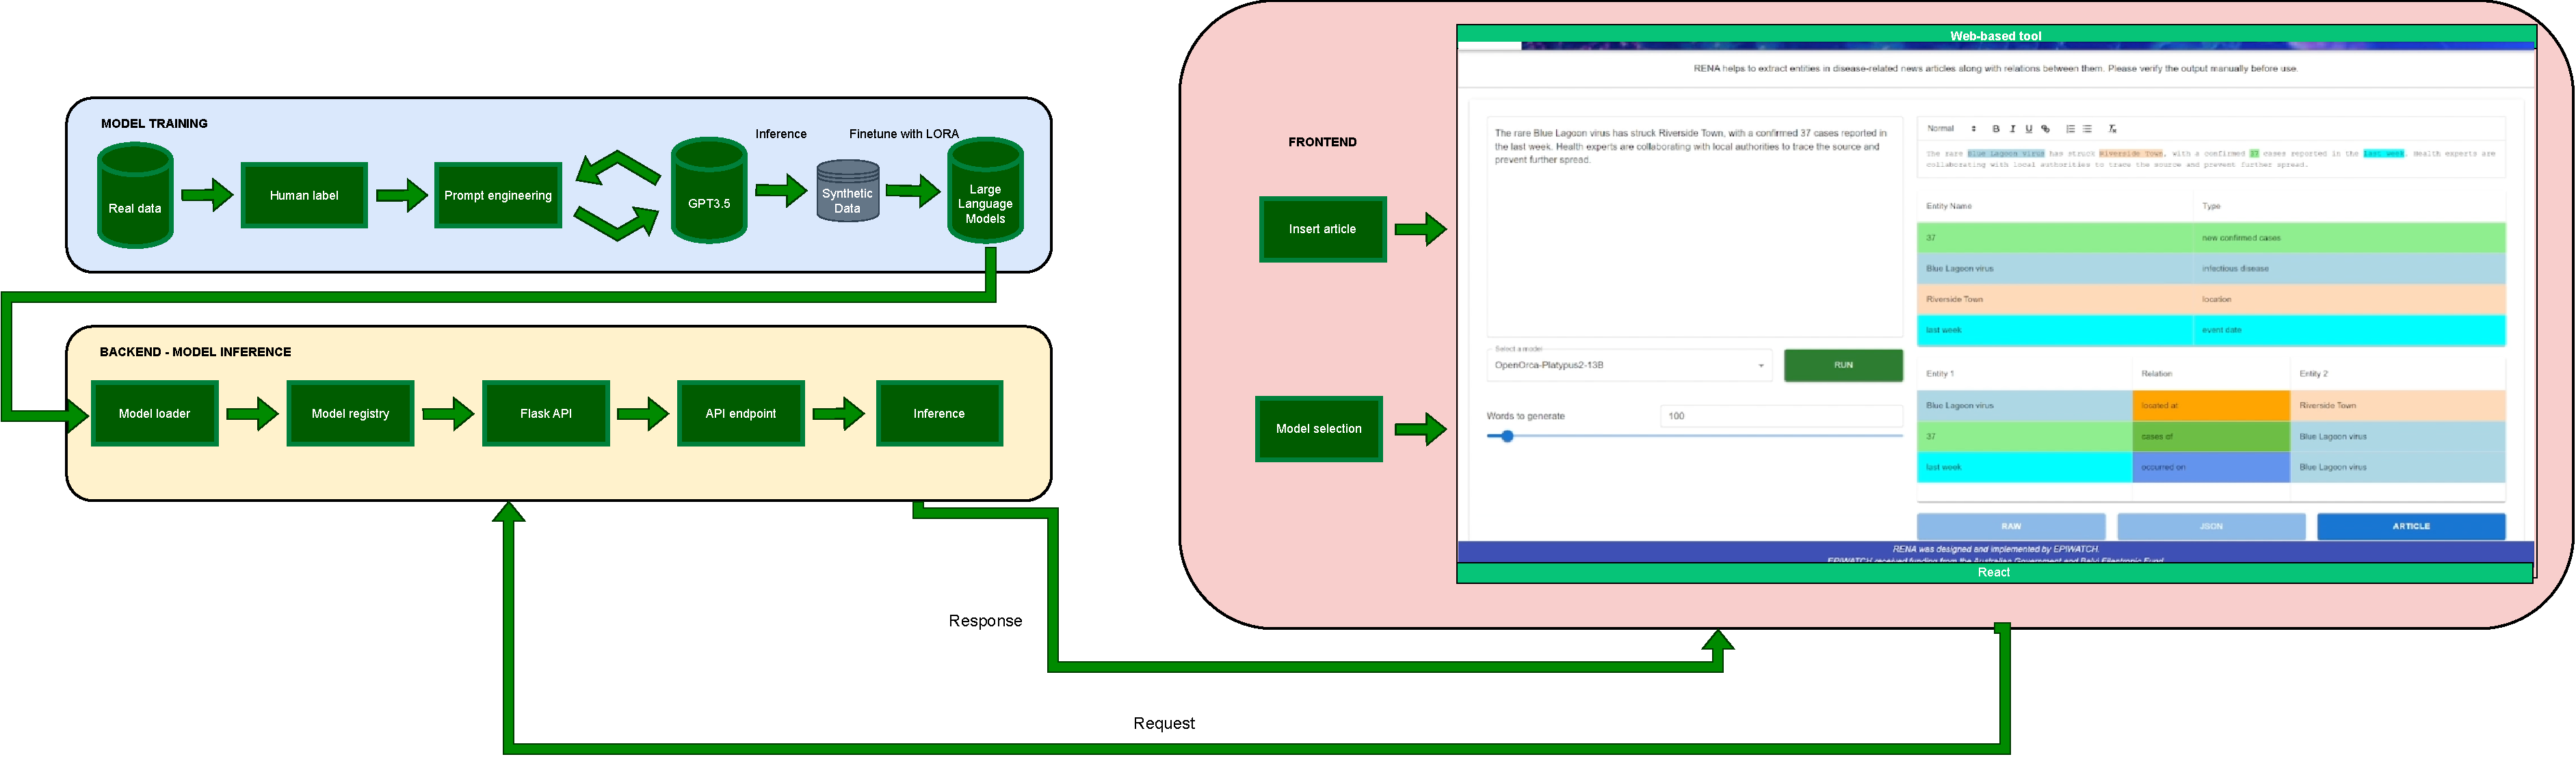
\includegraphics[width=1.0\textwidth, height=0.25\textheight]{figs/aaai3.pdf}
\caption{Architecture}
\label{fig:architecture}
\end{figure*}

\section{Architecture}
Figure~\ref{fig:architecture} shows the architecture of RENA. In the model training phase, we generated a set of 300 synthetic articles, annotated with relevant entities and relationships using 1-shot prompting with OpenAI API~\footnote{?; Accessed on 3rd October, 2023.} (gpt-3.5-turbo-16k) (Details in Supplementary Document.). The generated output (articles, and labeled entities and relations) were used for fine-tuning two large language models including \texttt{OpenOrca-Platypus2-13B}\footnote{\url{https://huggingface.co/Open-Orca/OpenOrca-Platypus2-13B}; Accessed on 3rd October, 2023.} and \texttt{Mythical-Destroyer-V2-L2-13B}\footnote{\url{https://huggingface.co/Sao10K/Mythical-Destroyer-V2-L2-13B}; Accessed on 3rd October, 2023.}, both based on Meta's LLaMa2 13B model~\cite{touvron2023llama}, using quantized low-rank adaptation (QLoRa)~\cite{dettmers2023qlora}. We run the training process for three epochs. In the inference phase, RENA allows for the selection of the two different models specified above. Our backend is built with Python Flask, where the model is both loaded and executed for inference. The output is then sent to our frontend, developed in React, to display the response.

We evaluated the two models included in RENA on 10 randomly selected articles in English, selected from the EPIWATCH database, an existing database with more than 1 million news articles relating to infectious disease outbreaks searched through online news, and prioritised using machine learning-based classification supplemented with manual curation by experts. We computed precision, recall and F1 score, comparing the predicted to labeled output on the ten articles for each model. We assessed the accuracy for named entity recognition (NER) and RE separately. RE was only evaluated for relevant entities that were recognised, so both metrics should be considered when assessing the models. Table~\ref{tab1} shows the precision, recall and F-score values for the models included in RENA.



\begin{table}[]
\begin{tabular}{lllll}
\toprule
 Model  & Eval & Precision &  Recall  &  F1  \\ \midrule
 Open-Orca-13b &  NER & 0.93 & 0.66 & 0.77 \\
 Open-Orca-13b  & RE  & 0.88 & 0.88 & 0.88 \\
 Mythical-Destroyer-13b  & NER & 0.96  & 0.57 & 0.71 \\
 Mythical-Destroyer-13b & RE & 0.97 & 0.97 & 0.97 \\ \bottomrule
\end{tabular}
\caption{Evaluation of models in RENA.}
\label{tab1}
\end{table}


\section{User Interface}

Figure 1 is a snapshot of the web interface hosting RENA. On the webpage includes:
\begin{itemize}
    \item \textbf{Input:} The input contains the text field that the user can input their unstructured article into, from which the model will extract entities and relations.
    \item \textbf{Select Model:} The select model box contains a dropdown to select between the 2 models to be used for generation.
    \item \textbf{Submit:} Begins the generation process.
    \item \textbf{Max tokens:} Max tokens is a slider to determine how many tokens of output will be produced by the model.
    \item \textbf{Output:} The model will generate the output (relations) into this box.
    \item \textbf{Raw Button:} The raw generated output of the model will be displayed in the output box when clicked.
    \item \textbf{JSON Button:} The output will be converted into a JSON format and be displayed in the output box when clicked.
    \item \textbf{Article Button:} The article will be displayed in the output box and the entities will be highlighted in the text and color coded. A table showing all the entity and entity types as well as another table showing the relations will also be shown.
\end{itemize}


\section{Summary \& Future Work}
RENA is a tool that uses QLoRA to finetune LLMs and extract disease-related relations from news articles. It offers a way to automate the creation of structured data from an inputted unstructured news article and output relatively accurate results. RENA will enable users interested in researching diseases to parse large amounts of data to potentially aid in the surveillance and prevention of diseases. We plan to extend RENA to multilingual news articles. In addition, different relations can help delineate different disease events, allowing detection of independent outbreaks involving different infections or locations from news articles.
Nostrum a sequi qui necessitatibus ex dolorem, delectus suscipit quasi fugiat, voluptatum illum nobis beatae ea hic eligendi tempore ipsam facilis tempora consequuntur, tempora quia tempore provident exercitationem beatae aut nisi minus assumenda molestias accusamus?\clearpage
\bibliography{aaai24}

\end{document}



